\documentclass[11pt]{beamer}
\usetheme{Madrid}
\usecolortheme{crane}

\title{Síkgeometria}
\author{Botló Bence Balázs}
\institute{Selye János Egyetem}
\date{\today}

\usepackage{enumitem}
\usepackage{graphicx}

\begin{document}
\frame{\maketitle}
\frame{\tableofcontents}
\begin{frame}[<+->]
\frametitle{Thalész-tétel}
\begin{block}{\textbf{Thalész-tétel}}
\begin{itemize}[label=$\circ$]
\item A Thalész-tétel és megfordítása: Egy háromszög akkor és csak akkor derékszögű, ha köré írható körének középpontja az egyik oldalának felezőpontja.
\end{itemize}
\end{block}
\end{frame}

\section{\textbf{Magasságtétel, befogótétel}}
\begin{frame}[<+->]
\begin{block}{\textbf{Magasságtétel, befogótétel}}
\frametitle{Magasságtétel, befogótétel}
\begin{itemize}[label=$\circ$]
\item Magasságtétel: Egy derékszögű háromszög magasságának hossza mértani közepe azon két szakasz hosszának, amelyekre a magasság az átfogót osztja.
\item Befogótétel: Egy derékszögű háromszög befogójának hossza mértani közepe az átfogó és a befogó átfogóra eső merőleges vetülete hosszának.
\end{itemize}
\end{block}
\end{frame}

\begin{frame}
\frametitle{Derékszögű háromszög}
\begin{figure}
  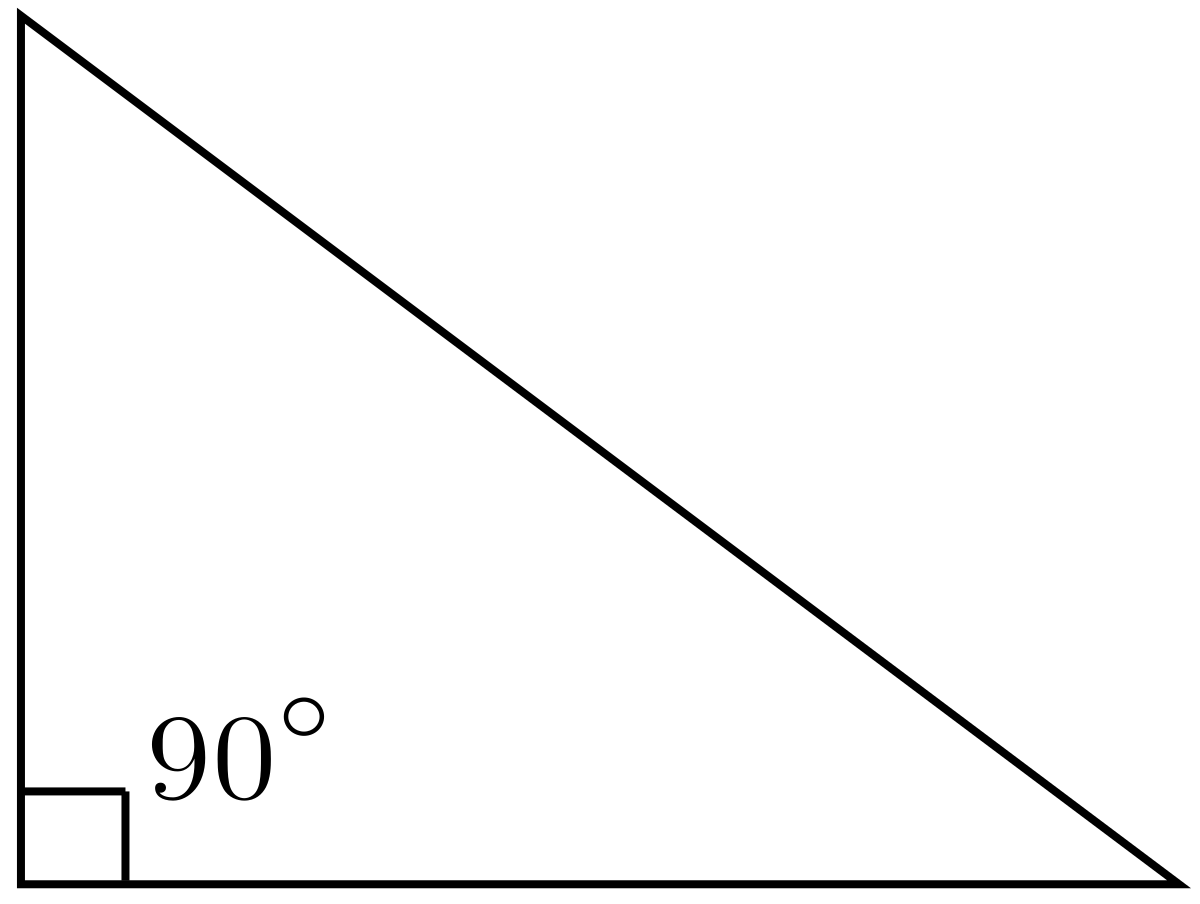
\includegraphics[width=0.8\textwidth]{right_triangle.png}
\end{figure}
\end{frame}

\section{\textbf{A háromszög néhány további területképlete}}
\begin{frame}[<+->]
\frametitle{Háromszög}
\begin{block}{\textbf{A háromszög néhány további területképlete}}
\begin{list}{}{\leftmargin=1.5em}
\item Jelölje $a$, $b$, $c$ a háromszög oldalainak hosszát, $\alpha$, $\beta$, $\gamma$ a megfelelő belső szögeket, $m_a, m_b, m_c$, a magasságok hosszait, \textit{s} a kerület felét és \textit{R} a köré írható kör sugarát!
\end{list}
\begin{itemize}
\item $ t = \frac{a \cdot m_a}{2} = \frac{b \cdot m_b}{2} = \frac{c \cdot m_c}{2}$.
\item $ t = \frac{a \cdot b \cdot \sin\!\gamma} {2} = \frac{b \cdot c \cdot \sin\!\alpha} {2} = \frac{a \cdot c \cdot \sin\!\beta} {2}$.
\item $t = \frac{a^2 \cdot \sin\!\beta \cdot \sin\!\gamma}{2 \cdot \sin\!\alpha}$.
\item $t = 2 \cdot R^2 \cdot \sin\!\alpha \cdot \sin\!\beta \cdot \sin\!\gamma$.
\item $t = \frac{R^2}{2} \cdot (\sin\!2\alpha + \sin\!2\beta + \sin\!2\gamma)$.
\item $t = \sqrt{s(s-a)(s-b)(s-c)}$, Heron-képlet.
\end{itemize}
\end{block}
\end{frame}

\section{\textbf{Trapéz}}
\begin{frame}[<+->]
\frametitle{Trapéz}
\begin{block}{\textbf{Trapéz}}

\begin{itemize}[label=$\circ$]
\item A négyszög belső szögeinek összege $360^\circ$ .
\end{itemize}
\begin{itemize}[label=$\circ$]
\item Ha egy négyszögnek van két párhuzamos oldala, akkor \textbf{trapéznak} nevezzük.
\item A trapéz párhuzamos oldalait \textbf{alapoknak}, a másik két oldalát \textbf{száraknak} nevezzük.
\item A \textbf{trapéz magassága} az alapokat merőlegesen összekötő szakasz. (az alapok távolsága)
\item A \textbf{trapéz középvonala} a szárak felezőpontjait összekötő szakasz.
\item A trapéz szárainak felezőpontjait összekötő középvonala párhuzamos az alapokkal, hossza pedig az alapok hosszainak számtani közepe.
\item A trapézban az egy száron fekvő szögek összege 180 fok. (társszögek)
\item A \textbf{trapéz derékszögű}, ha van derékszöge.
\end{itemize}
\end{block}
\end{frame}

\begin{frame}[<+->]
\frametitle{Trapéz}
\begin{block}{\textbf{Trapéz 2}}
\begin{itemize}[label=$\circ$]
\item A \textbf{trapéz egyenlő szárú}, ha szárai egyenlő hosszúak.
\item Ha egy trapéz tengelyesen szimmetrikus, akkor \textbf{szimmetrikus trapéznak} nevezzük
\item A szimmetrikus trapéz alapon fekvő szögei egyenlők.
\item Minden szimmetrikus trapéz egyenlő szárú, de nem minden egyenlő szárú trapéz szimmetrikus.
\item A szimmetrikus trapézok köré kör írható (húrtrapéz).
\item A szimmetrikus trapéz szimmetria-tengelye felezi az alapokat és merőleges azokra.
\item A trapéz területét megkapjuk, ha az alapok hosszainak számtani közepét megszorozzuk a trapéz magasságának hosszával.
\end{itemize}
\end{block}
\end{frame}

\begin{frame}
\frametitle{Trapéz}
\begin{figure}
  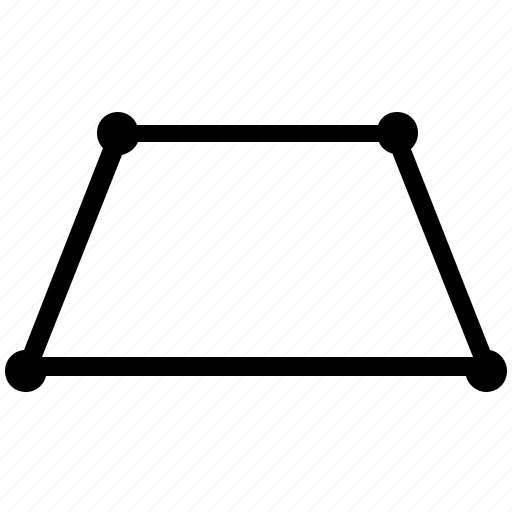
\includegraphics[width=0.8\textwidth]{trapeze.png}
\end{figure}
\end{frame}

\section{\textbf{Paralelogramma}}
\begin{frame}[<+->]
\frametitle{Paralelogramma}
\begin{block}{\textbf{Paralelogramma}}
\begin{itemize}[label=$\circ$]
\item Ha egy négyszög szemközti oldalai párhuzamosak, akkor \textbf{paralelogrammának} nevezzük.
\item Egy négyszög akkor és csak akkor paralelogramma, ha
\begin{itemize}[label=$\cdot$]
\item szemközti szögei egyenlők;
\item az egy oldalon fekvő szögeinek összege $180^\circ$;
\item szemközti oldalai egyenlők;
\item ha van két szemközti oldala, amelyek egyenlők és párhuzamosak;
\item középpontosan szimmetrikus;
\item átlói felezik egymást.
\end{itemize}
\end{itemize}
\end{block}
\end{frame}

\begin{frame}[<+->]
\frametitle{Paralelogramma}
\begin{block}{\textbf{Paralelogramma 2}}
\begin{itemize}[label=$\circ$]
\item A paralelogramma két szemközti oldalának felezési pontjait összekötő szakaszt a \textbf{paralelogramma} középvonalának nevezzük.
\item A paralelogramma két szemközti oldalának felezési pontjait összekötő középvonala párhuzamos a másik két oldallal és velük egyenlő hosszú.
\item A paralelogramma adott oldalához tartozó \textbf{magassága} a szemközti oldal egy pontjából az
adott oldal egyenesére bocsátott merőleges szakasz.
\item A paralelogramma területét megkapjuk, ha egyik oldalának hosszát megszorozzuk a hozzá tartozó magasság hosszával.
\end{itemize}
\end{block}
\end{frame}

\begin{frame}
\frametitle{Paralelogramma}
\begin{figure}
  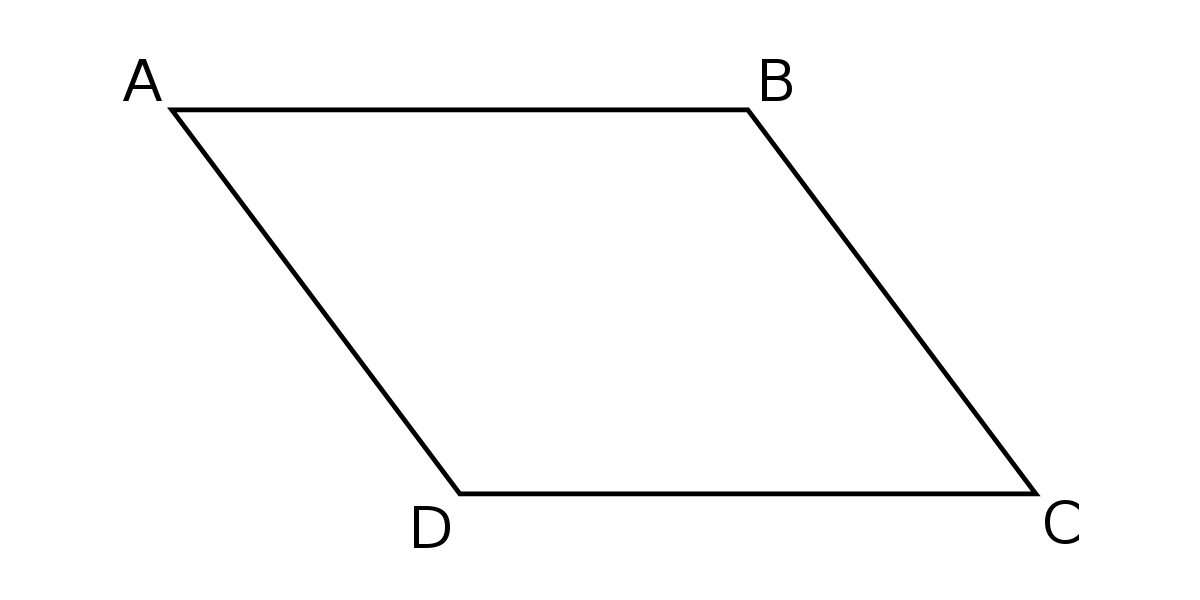
\includegraphics[width=0.8\textwidth]{paralelogram.png}
\end{figure}
\end{frame}

\section{\textbf{Deltoid}}
\begin{frame}[<+->]
\frametitle{Deltoid}
\begin{block}{\textbf{Deltoid}}
\begin{itemize}[label=$\circ$]
\item Ha egy négyszög valamelyik átlójára tengelyesen szimmetrikus, akkor \textbf{deltoidnak} nevezzük.
\item A deltoid átlói merőlegesek egymásra.
\item A deltoid szimmetriaátlója felezi a másik átlót.
\item A deltoidnak két-két szomszédos oldala egyenlő hosszú.
\item A deltoid szimmetriaátlóval szemközti szögei egyenlők.
\item Van konkáv deltoid is.
\item A deltoid területe egyenlő az átlók hosszai szorzatának felével.
\end{itemize}
\end{block}
\end{frame}

\begin{frame}
\frametitle{Deltoid}
\begin{figure}
  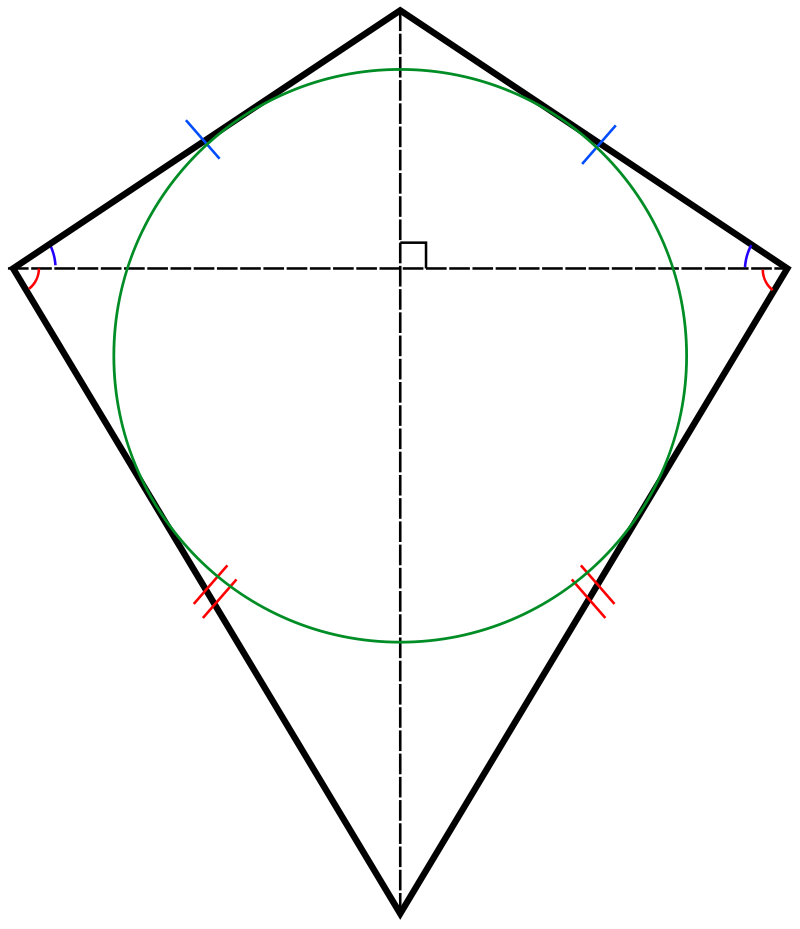
\includegraphics[width=0.5\textwidth]{deltoid.png}
\end{figure}
\end{frame}

\section{\textbf{Rombusz}}
\begin{frame}[<+->]
\frametitle{Rombusz}
\begin{block}{\textbf{Rombusz}}
\begin{itemize}[label=$\circ$]
\item Ha egy négyszög oldalai egyenlő hosszúak, akkor \textbf{rombusznak} nevezzük.
\item Minden rombusz paralelogramma is (tehát rendelkezik a paralelogramma összes tulajdonságával).
\item Minden rombusz deltoid is (tehát rendelkezik a deltoid összes tulajdonságával).
\end{itemize}
\end{block}
\end{frame}

\begin{frame}
\frametitle{Rombusz}
\begin{figure}
  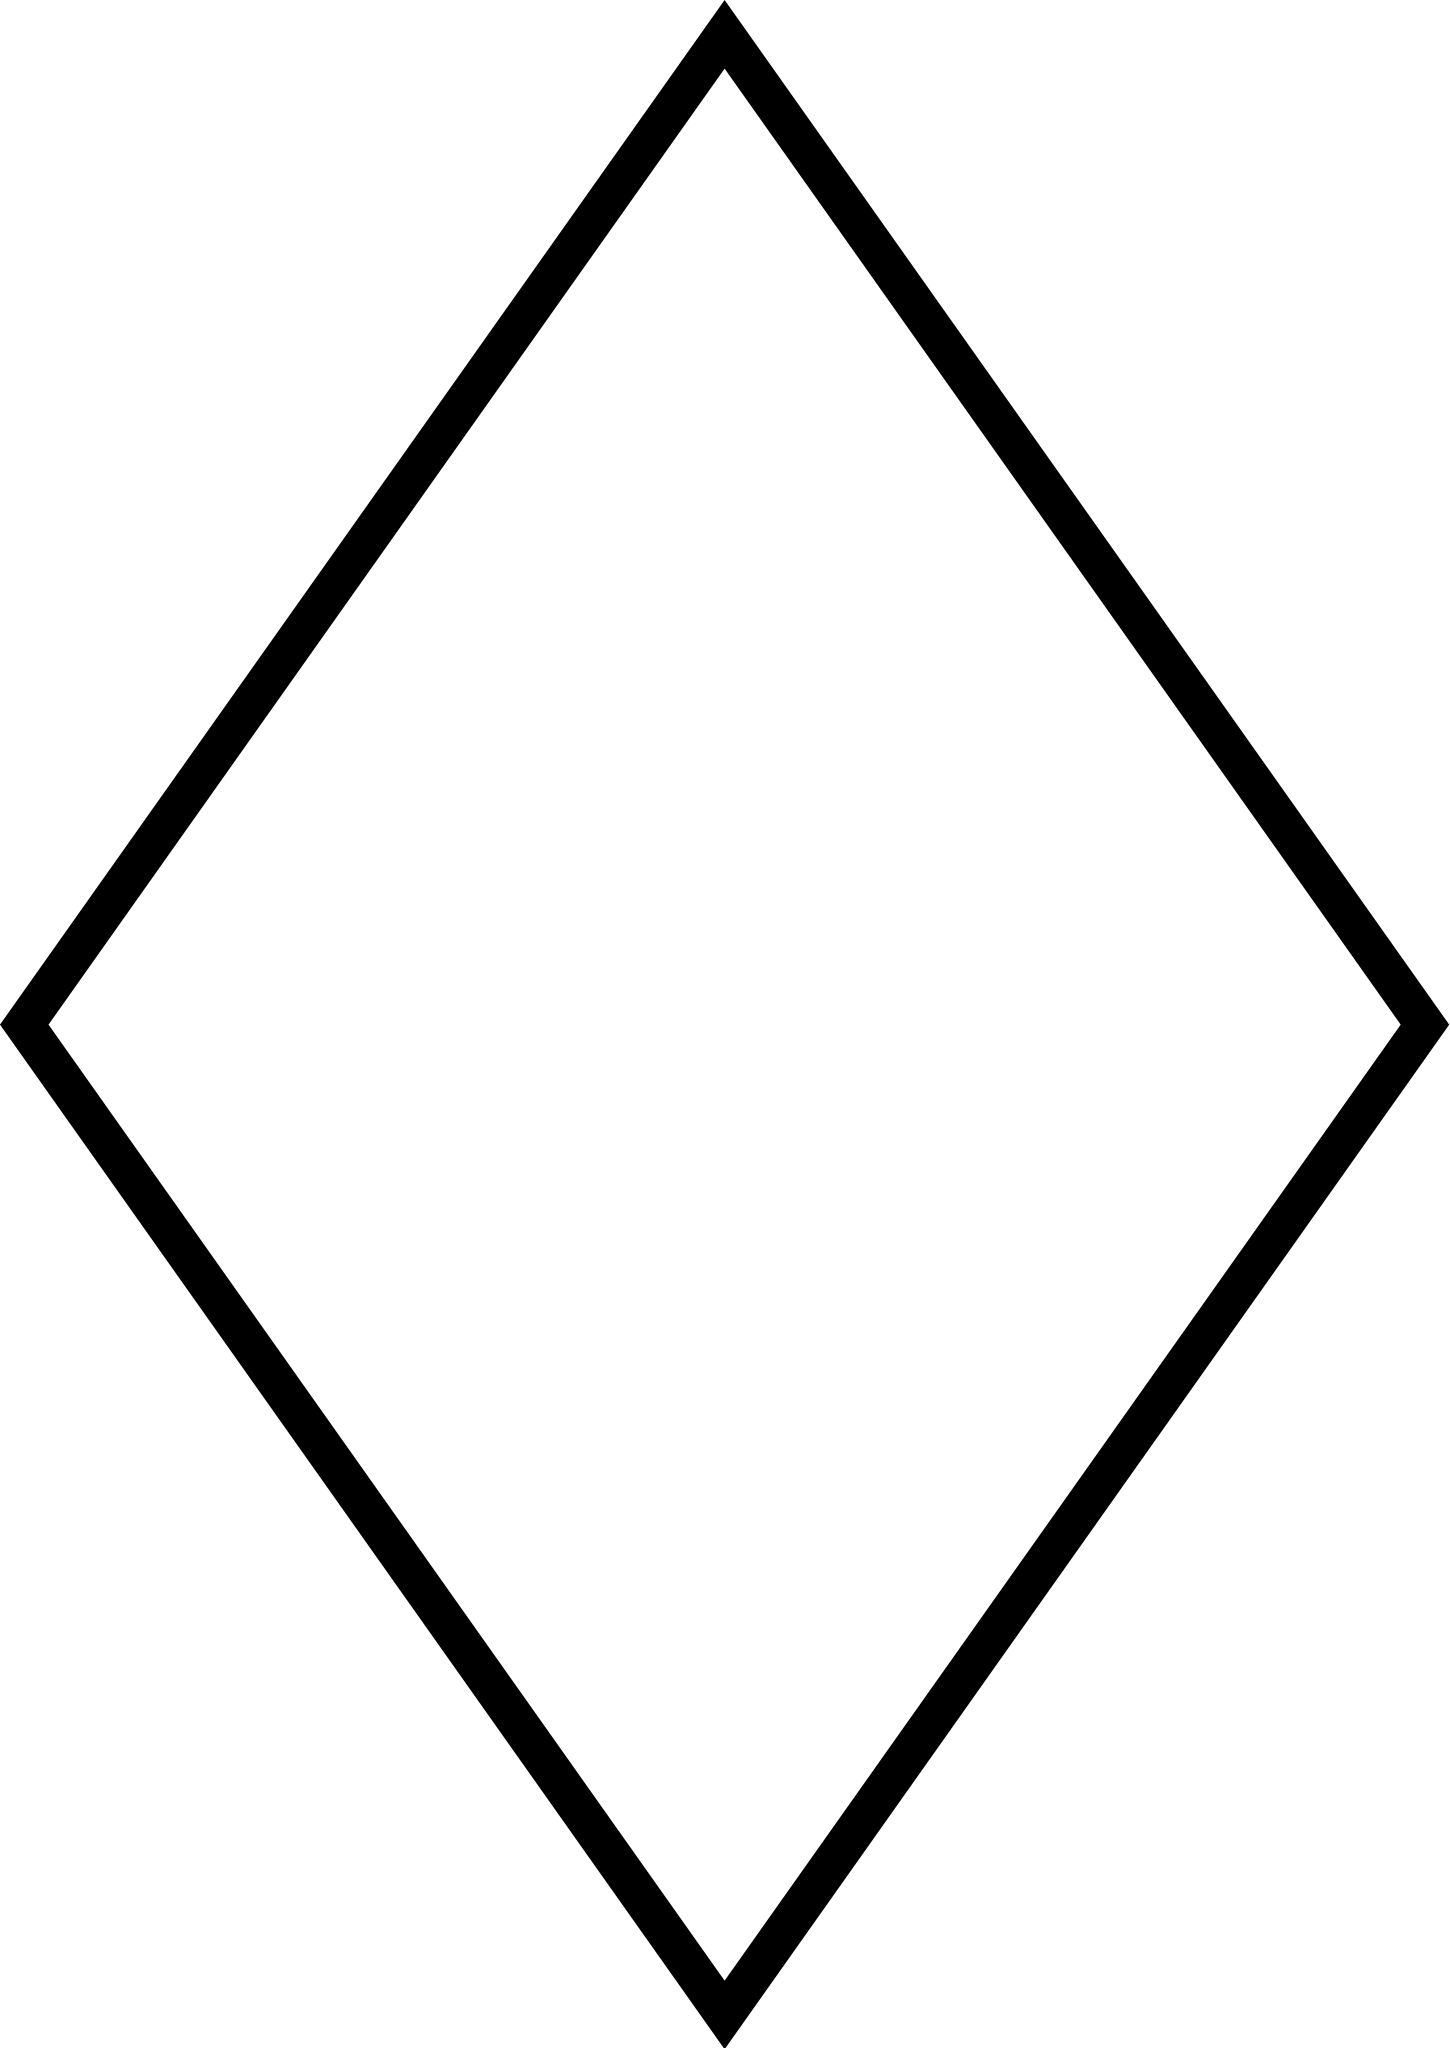
\includegraphics[width=0.4\textwidth]{rhombus.png}
\end{figure}
\end{frame}

\section{\textbf{Téglalap}}
\begin{frame}[<+->]
\frametitle{Téglalap}
\begin{block}{\textbf{Téglalap}}
\begin{itemize}[label=$\circ$]
\item Ha egy négyszög szögei egyenlők, akkor \textbf{téglalapnak} nevezzük.
\item A téglalap szögei 90 fokosak
\item A téglalap
\begin{itemize}[label=$\cdot$]
\item szemközti oldalai egyenlők és párhuzamosak egymással;
\item átlói felezik egymást;
\item középpontosan szimmetrikus az átlók felezéspontjára nézve;
\item tengelyesen szimmetrikus a szemközti oldalfelező pontokon átmenő egyenesekre.
\end{itemize}
\item A téglalap területe egyenlő az egy csúcsában összefutó oldalak hosszainak szorzatával.
\item Minden téglalap húrtrapéz, derékszögű trapéz, paralelogramma is.
\end{itemize}
\end{block}
\end{frame}

\begin{frame}
\frametitle{Téglalap}
\begin{figure}
  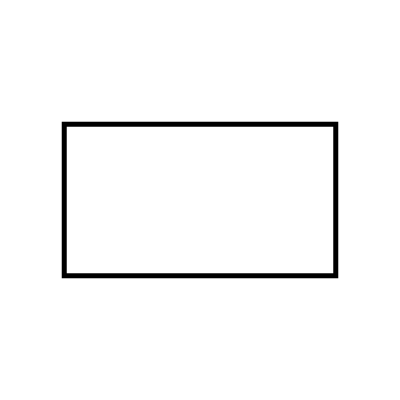
\includegraphics[width=0.8\textwidth]{rectangle.png}
\end{figure}
\end{frame}

\section{\textbf{Négyzet}}
\begin{frame}[<+->]
\frametitle{Négyzet}
\begin{block}{\textbf{Négyzet}}
\begin{itemize}[label=$\circ$]
\item Ha egy négyszög minden oldala egyenlő hosszú és minden szöge egyenlő, akkor \textbf{négyzetnek} nevezzük.
\item A négyzet területe egyenlő oldalhosszának négyzetével.
\item Egy négyszög két középvonala felezve metszi egymást.
\end{itemize}
\end{block}

\begin{block}{\textbf{Érintőnégyszögek}}
\begin{itemize}[label=$\circ$]
\item Azokat a négyszögeket, amelyeknek van beírt körük, \textbf{érintőnégyszögeknek} nevezzük.
\item Egy konvex négyszög akkor és csak akkor érintőnégyszög, ha a szemközti oldalak hosszainak összege egyenlő.
\item Az érintőnégyszög területét úgy is megkaphatjuk, ha beírt körének sugarát megszorozzuk a kerület felével.
\end{itemize}
\end{block}
\end{frame}

\begin{frame}[<+->]
\frametitle{Négyzet}
\begin{block}{\textbf{Húrnégyszögek}}
\begin{itemize}[label=$\circ$]
\item Azokat a négyszögeket, amelyeknek van körülírt körük, \textbf{húrnégyszögeknek} nevezzük.
\item Egy négyszög akkor és csak akkor húrnégyszög, ha szemközti szögeinek összege $180^\circ$.
\item Ptolemaiosz-tétel: A húrnégyszög átlóinak szorzata egyenlő a szemközti oldalpárok szorzatának összegével.
\end{itemize}
\end{block}
\end{frame}

\begin{frame}
\frametitle{Négyzet}
\begin{figure}
  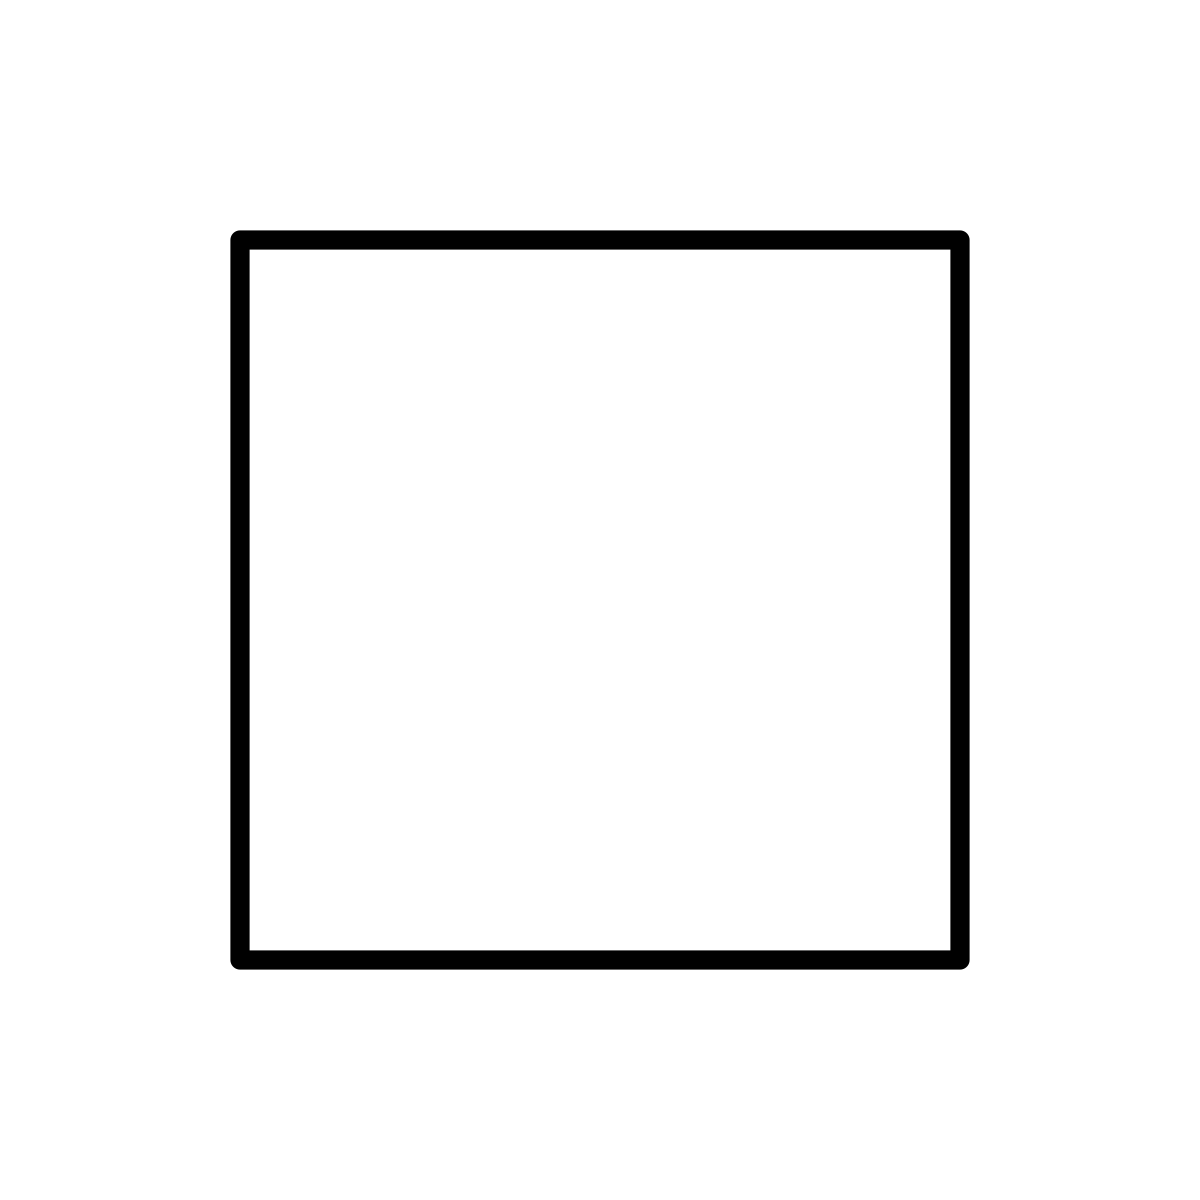
\includegraphics[width=0.8\textwidth]{square.png}
\end{figure}
\end{frame}

\section{\textbf{Sokszögek}}
\begin{frame}[<+->]
\frametitle{Sokszög}
\begin{block}{\textbf{Sokszögek}}
\begin{itemize}[label=$\circ$]
\item Egy \textbf{sokszög konvex}, ha minden szöge konvex, egy \textbf{sokszög konkáv}, ha van konkáv szöge.
\item Az n-oldalú konvex sokszög átlóinak száma: $\frac{n(n-3)}{2}$.
\item Az n-oldalú sokszög belső szögeinek összege: $(n-2) \cdot 180^\circ$
\item Egy sokszög szabályos, ha minden oldala egyenlő hosszú, és minden szöge egyenlő nagyságú.
\end{itemize}
\end{block}
\end{frame}

\begin{frame}
\frametitle{Sokszögek}
\begin{figure}
  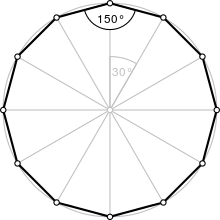
\includegraphics[width=0.6\textwidth]{dodecagon.png}
\end{figure}
\end{frame}

\section{\textbf{Kör és részei, körív hossza, körcikk területe}}
\begin{frame}[<+->]
\frametitle{Kör}
\begin{block}{\textbf{Kör és részei, körív hossza, körcikk területe}}
\begin{itemize}[label=$\circ$]
\item A \textbf{kör} azon pontok halmaza a síkon, amelyek a sík egy adott O pontjától adott $r$ távolságra vannak.
\item A kör két különböző pontját összekötő szakaszt \textbf{húrnak}, a húrt tartalmazó egyenest \textbf{szelőnek} nevezzük.
\item A kör középpontján átmenő húrt \textbf{átmérőnek} nevezzük.
\item A kört két különböző pontja két \textbf{körívre} osztja fel.
\item A körlap azon részét, amelyet a kör egy íve és az ív végpontjaiba húzott sugarak határolnak, \textbf{körcikknek} nevezzük.
\item A körlap azon részét, amelyet a kör egy íve és az ív végpontjait összekötő húrja határolnak, \textbf{körszeletnek} nevezzük.
\item A sík két koncentrikus köre által közrefogott részét \textbf{körgyűrűnek} nevezzük.
\item A \textbf{kör érintője} a kör síkjának olyan egyenese, amelynek egyetlen közös pontja van a körrel.
\item A kör érintője merőleges az érintési pontba húzott sugárra.
\end{itemize}
\end{block}
\end{frame}

\begin{frame}[<+->]
\frametitle{Kör}
\begin{block}{\textbf{Kör és részei, körív hossza, körcikk területe 2}}
\begin{itemize}[label=$\circ$]
\item Egy külső pontból a körhöz húzott két érintőszakasz egyenlő hosszú.
\item (Körhöz húzott érintő- és szelőszakaszok tétele) Adott körhöz adott külső pontból húzott érintőszakaszok hossza mértani közepe azon két szakasz hosszának, amelyek az adott ponton átmenő szelőn a ponttól a körrel alkotott metszéspontokig terjednek.
\item (Körhöz külső pontból húzott szelőszakaszok tétele) Adott körhöz adott külső ponton át húzott szelőn az adott ponttól a körrel alkotott metszéspontokig terjedő szelőszakaszok hosszának szorzata állandó, csak a körtől és az adott ponttól függ.
\item Adott körhöz adott belső pontján át húzott szelőn az adott ponttól a körrel alkotott metszéspontokig terjedő szelőszakaszok hosszának szorzata állandó, csak a körtől és az adott ponttól függ.
\item Ha egy szög csúcsa egy adott kör középpontja, akkor középponti szögnek nevezzük.
\end{itemize}
\end{block}
\end{frame}

\begin{frame}[<+->]
\frametitle{Kör}
\begin{block}{\textbf{Kör és részei, körív hossza, körcikk területe 3}}
\begin{itemize}[label=$\circ$]
\item Egy körben a középponti szögek nagysága és a hozzájuk tartozó körívek hosszai egyenesen arányosak. $\frac{\alpha}{\beta} = \frac{i_\alpha}{i_\beta}$.
\item Ívmérték: \textbf{1 radián} az szög, amelyhez mint középponti szöghöz a kör sugarával egyenlő hosszú körív tartozik. $\pi$ radián $= 180^\circ$.
\item Adott $r$ sugarú körben az $\alpha$ középponti szöghöz tartozó körív hossza:
\begin{center}
$i_{\alpha^\circ} = \frac{r\pi}{180^\circ}\alpha$, illetve $i_{\hat{\alpha}} = r\hat{\alpha}$.
\end{center}
\item Egy körben a középponti szögek nagysága és a hozzájuk tartozó körcikkek területei egyenesen arányosak. $ \frac{\alpha}{\beta} = \frac{t_\alpha}{t_\beta}$.
\item Adott $r$ sugarú körben az $\alpha$ középponti szöghöz tartozó körcikk területe:
\begin{center}
$t_{a^\circ} = \frac{r^2\pi}{360^\circ}\alpha$, illetve $t_{\hat{a}}=$  $\frac{^i\hat{a}^r}{2}$.
\end{center}
\end{itemize}
\end{block}
\end{frame}

\begin{frame}
\frametitle{Kör}
\begin{figure}
  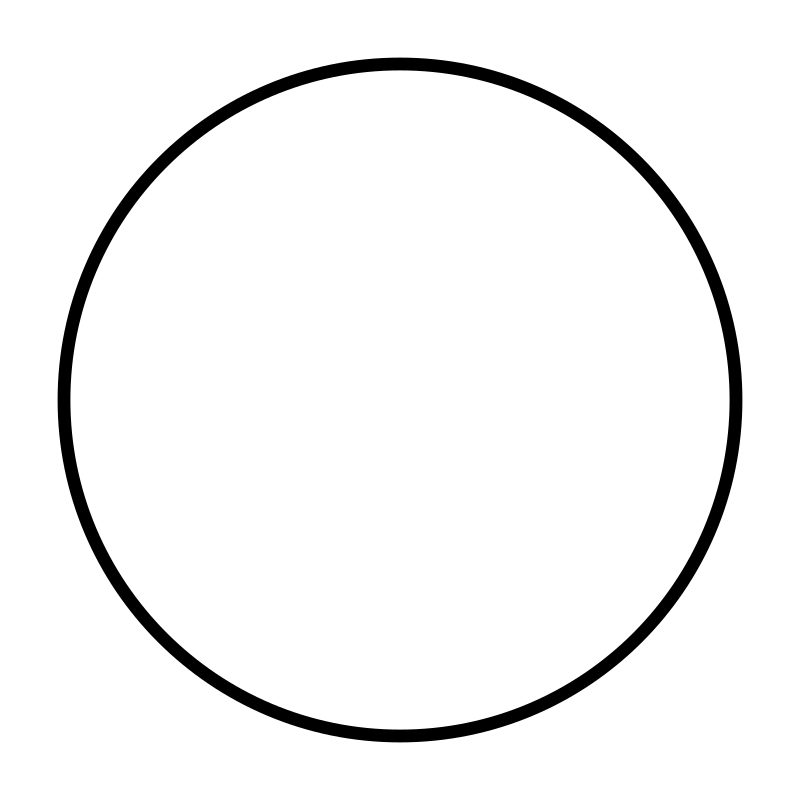
\includegraphics[width=0.6\textwidth]{circle.png}
\end{figure}
\end{frame}

\section{\textbf{Kerületi szögek, látókör}}
\begin{frame}[<+->]
\frametitle{Kerületi szögek, látókör}
\begin{block}{\textbf{Kerületi szögek, látókör}}
\begin{itemize}[label=$\circ$]
\item Ha egy szög csúcsa egy adott körvonal pontja, szárai pedig vagy a kör két húrjára, vagy egy húrra és egy érintőre illeszkednek, akkor a kör \textbf{kerületi szögének} nevezzük. Ha a kerületi szög egyik szára egy érintőre illeszkedik, akkor \textbf{érintőszárú kerületi szögnek} nevezzük.
\item (Kerületi és középponti szögek tétele) Egy körben egy adott ívhez tartozó középponti szög kétszerese az ugyanazon ívhez tartozó kerületi szögnek.
\item (Kerületi szögek tétele) Egy körben egy adott ívhez tartozó kerületi szögek egyenlők.
\end{itemize}
\end{block}
\end{frame}

\begin{frame}[<+->]
\frametitle{Kerületi szögek, látókör}
\begin{block}{\textbf{Kerületi szögek, látókör 2}}
\begin{itemize}[label=$\circ$]
\item (Látószög-körív; látókör) A síkon azoknak a pontoknak a halmaza, amelyekből egy adott $AB$ szakasz adott $(0^\circ < \alpha < 180^\circ)$ szögben látszik, két szimmetrikus körív.
\begin{itemize}[label=$\circ$]
\item Az $AB$ szakasz  a két körív közös húrja, és az $A$ és $B$ pontok nem tartoznak a látószögkörívhez.
\item (Thalész-tétel) Adott kör egy tetszőleges $AB$ átmérője a kör bármely $A$-tól és $B$-től különböző pontjából derékszögben látszik.
\item (A Thalész-tétel megfordítása) Ha egy háromszög $AB$ oldala a szemközti $C$ csúcsból derékszögben látszik, akkor a $C$ csúcs az $AB$ átmérőjű kör $A$-tól és $B$-től különböző pontja.
\end{itemize}
\end{itemize}
\end{block}
\end{frame}
\end{document}